\section{Selecteren methoden, technieken en tools}

Een ontwikkelstraat staat aan de basis van succesvolle softwareontwikkeling, en zorgt voor een duidelijke structuur tijdens de ontwikkeling van het Proof of Concept. Hierbij wordt er gebruik gemaakt van de \gls{OTAP} aanpak, waarbij er voor elke fase van het ontwikkeltraject een omgeving beschikbaar is.

\subsection{Programmeertaal}

In de opdrachtformulering zoals beschreven door Quintor, te vinden in bijlage \ref{appendix:opdrachtformulering}, zijn er twee keuzes voor de programmeertaal voorgesteld, C\# of Java, waarmee het Proof of Concept gerealiseerd dient te worden. Zelf heb ik met beide talen ervaring opgedaan tijdens de studie, waardoor beide talen een mogelijke keuze zijn. Aangezien mijn begeleider vanuit Quintor een Java ontwikkelaar is, neigt de keuze al snel naar desbetreffende taal. Dit omdat er altijd de mogelijkheid is om hem te benaderen wanneer er Java expertise benodigd is. Zelf ben ik niet enthousiast over Java en bleek de andere afstudeerder waarmee er een mate van overlap is tussen de keuze voor de taal waarin het Proof of Concept gerealiseerd wordt dat ook niet te zijn. Alhoewel Java de meest voor hand liggende keuze is, hebben wij een voorstel gedaan aan de begeleider om gebruik te maken van de programmeertaal Kotlin.

\subsubsection{Kotlin}

Kotlin is een programmeertaal ontwikkeld door Jetbrains, een bedrijf dat bekend staat om hun wijde assortiment aan \acrfull{IDE}'s. Ze zochten een nieuwe programmeertaal die een verbetering op Java zou zijn, maar nog steeds compatible is voor migratiedoeleinden. Naar aanleiding hiervan heeft Jetbrains een team opgezet dat zich bezig ging houden met het ontwikkelen van deze nieuwe programmeertaal. Deze programmeertaal is Kotlin geworden en heeft in februari 2016 een 1.0 release gehad. De programmeertaal is volledig open-source en compileert naar de \acrfull{JVM}, waardoor Java en Kotlin tegelijkertijd gebruikt kunnen worden. Dit is een belangrijk punt aangezien dit betekend dat alle libraries die beschikbaar zijn voor Java, ook gebruikt kunnen worden in Kotlin \citep{mediaan_kotlin}.

Het doel van het gebruiken van Kotlin is dan ook om de adoptiesnelheid, de werking, en de ervaring aan te tonen aan Quintor, zodat ze kunnen overwegen om deze programmeertaal in te zetten in toekomstige projecten. In overleg met de bedrijfsbegeleider is dit goed bevonden.

\subsection{Versiebeheer}

In het hoofdstuk ``\nameref{organisatie:infrastructuur}'' is er gesproken over de versiebeheer die gebruikt wordt binnen Quintor. Het is dan ook een voor de hand liggende keuze dat BitBucket gebruikt wordt voor het waarborgen van de kwaliteit van de software, aangezien ik gebruik mag maken van de infrastructuur binnen Quintor. 

\subsection{Deployment}

\begin{wrapfigure}[11]{r}{0.4\textwidth}
    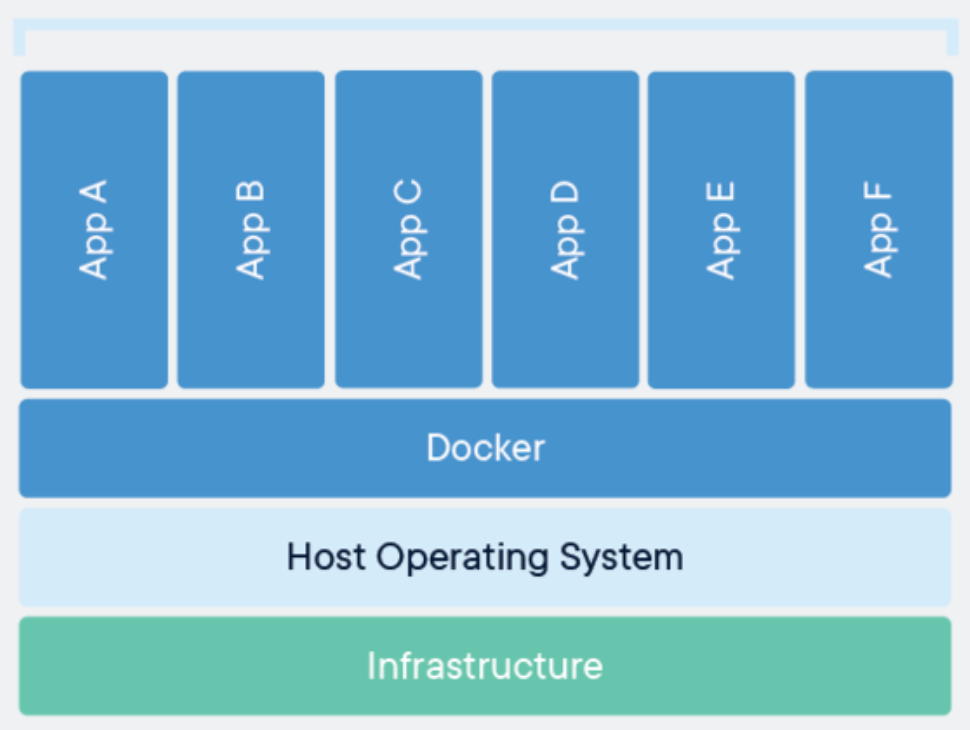
\includegraphics[width=0.4\textwidth, keepaspectratio]{figures/docker}
    \caption[Werking Docker]{Overzicht van de werking van Docker.}
    \label{realisation:docker}
\end{wrapfigure} 

Voor het inrichten van de \gls{OTAP} omgeving zal er gebruik gemaakt worden van containerisation. Deze optie is gekozen omdat er geen centraal deployment punt bestaat waarop de applicatie gedraaid kan worden. Gezien het feit dat de Blockchain per segment ontwikkeld wordt, is er veel baat bij overdraagbaarheid. Aangezien containerisation platformneutraal is, en dus op verschillende operating systems kan draaien, lijkt het mij een gepaste keuze om deze techniek toe te passen. De meest bekende technologie die containerisation faciliteert is Docker.

\subsubsection{Docker}

Een Docker container is een lichtgewicht, alleenstaand, uitvoerbaar pakket van software die alles bevat om een applicatie uit te voeren: code, een runtime, systeem tools, systeem libraries en settings. In fig. \ref{realisation:docker} is een overzicht te zien hoe Docker werkt. Hierin is te zien dat Docker gebruik maakt van het operating system van de computer waardoor er geen operating systeem per applicatie nodig is. Dit zorgt ervoor dat de technologie zeer efficiënt is.
